\section{Car-sharing systems} 
\label{sec:3_2_carsharing}

The first concepts of car-sharing systems date back to 1948, although the basic principles of such service were consolidated during the 1970s~\cite{harms1998emergence}.  The key idea behind car-sharing systems is that a fleet of cars is shared by several users that drive the cars whenever they need without owning it. Car-sharing differs from classic car rental because it is a self-service based service, and vehicles can be rented for shorter fractions of times (usually minutes). 
At the beginning of the 1990s, along with the emerging problems of large urban centers, high fuel prices, traffic congestion, high emission of pollutants, the idea of sharing vehicles started to become popular~\cite{becker2017comparing}. Since then, car sharing has been the subject of academy studies~\cite{millard2005car}. Understanding the dynamics of these services provides valuable insights into how people move in urban centers. This information can give support to precise and efficient urban planning, ranging from traffic planning or the design of communication infrastructures.

The car-sharing can be either station-based or the free-floating. The station-based can be divided into \textit{one-way services} and \textit{two-way services}. Station-based models require that a user pick up the vehicle she/he will use at a given base station. The user, in turn, may leave the vehicle at any of the base stations scattered throughout the service coverage region (i.e., one-way car-sharing service), or she/he may be obliged to return the vehicle to the station of origin (i.e., two-way car-sharing service). On one hand, the two-way model requires simpler logistics and infrastructure compared to other models. Its implementation can be performed faster and at a lower cost. 
On the other hand, the one-way model may be more flexible and cost-efficient to users than a classical rental. For example, in case there is a base station near to the final user destination, she/he may leave the car at the station while performing other tasks. The time the vehicle is parked is not charged, incurring to lower costs to users. However, a parked vehicle may be reserved by another user. 
The free-floating model does not require any fixed station. In other words, users reserve a car, parked into non-reserved spots in the streets. By the end of the use, users may leave vehicles at any location in a predefined area. Notably, free-floating model eliminates the limitations that station-based models hold, making the experience more flexible and closer to private-owned vehicles~\cite{ciari2014modeling}.

Figure~\ref{fig:diagrama} presents an abstract model that describes the possible states of a vehicle in any of the three car-sharing systems.
Intuitively, a car can be in use (i.e., \textit{busy}) or \textit{idle}. A \textit{busy} vehicle is \textit{rented}, meaning that someone is paying for it during this period. On the other hand, \textit{idle} vehicles may be \textit{unavailable} (i.e., during a maintenance process), \textit{available}, which means someone can reserve or it, or \textit{reserved}. 
% MC-old: More precisely, a vehicle is \textit{available} at the car-sharing system. In case a user pick-up this vehicle (i.e., rent it), its state changes from \textit{available} to \textit{rented}. In case a user reserves a vehicle, its state changes from \textit{available} to \textit{reserved}. Note that, a reservation of a vehicle is usually not charged and then, we consider this vehicle as idle.
% When a vehicle is \textit{available}, a user can pick-up it. In this case the status changes from \textit{available} to \textit{rented}. Instead if the users reserves the car (a preemption on the car with respect to the other users) the vehicle state switches from \textit{available} to \textit{reserved}. Note that a reservation of a vehicle is usually not charged and then, we consider this vehicle as idle.
% When \textit{reserved}, a user may pick-up the vehicle, and the vehicle status changes from \textit{reserved} to \textit{rented}. However, a user may also cancel a reservation and then the vehicle status goes back to \textit{available}.
% Without loss of generality, we consider a vehicle is \textit{unavailable} when it is either on maintenance or out of service.%) case it was previously available. %Finally, a vehicle in a given state may return to the previous one or, directly be stated as \textit{available}.
% As we will see in the next Section, not always the data contains the plain information about which of the four states the vehicle is. We will need to infer it by making some assumptions. 
The state in which the car is ready for a customer is \textit{available}. In this situation, the user can reserve the car and subsequently begins the ride or start to drive the vehicle instantaneously. In the first case the state changes from \textit{reserved} and then \textit{rented} while in the second case the state switches into \textit{rented} directly. When the customer concludes the rent the vehicle state moves from \textit{rented} to \textit{available} returning ready for another rent. Notice that if a user reserves the car and then cancels the reservation the vehicle state moves from \textit{reserved} to \textit{available} without assuming the state \textit{rented}. If a vehicle is not in one of the previous three states, then it is \textit{unavailable}, e.g., it is out of service. As we will see in the next Section, not always the data contains plain information about which of the four states the vehicle is. We will need to infer it by making some assumptions deducing the car state by filtering the rentals according to the duration and the possible driven distance.

\begin{figure}[tbh]
\centering
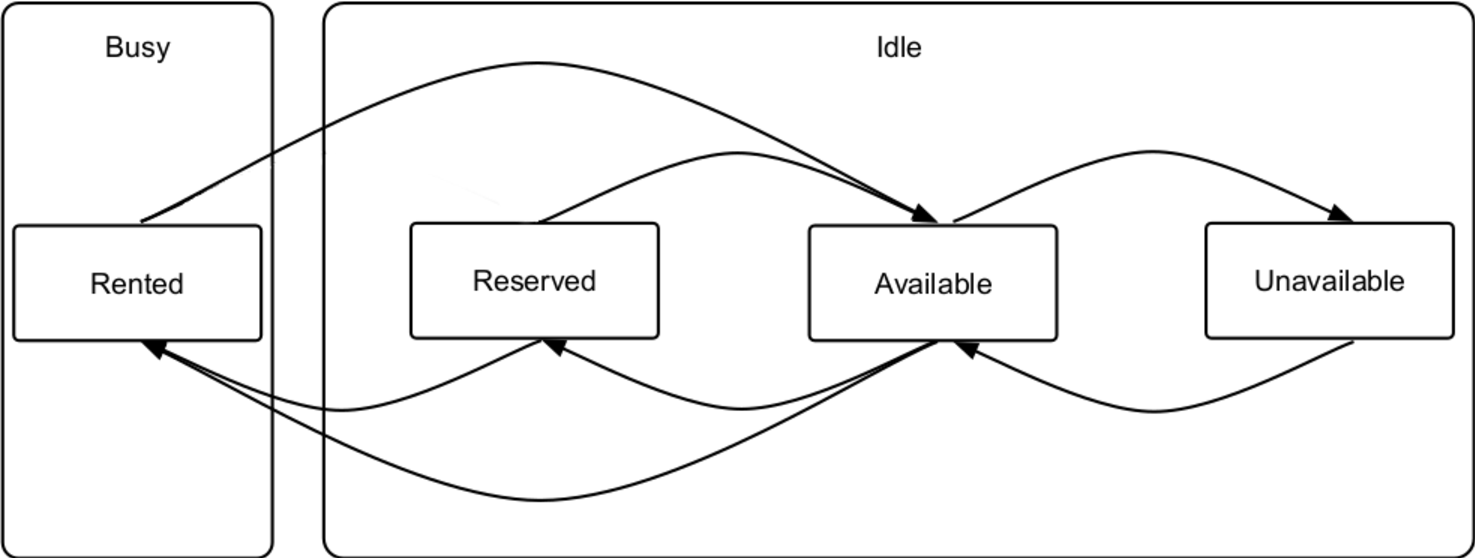
\includegraphics[width=1\textwidth]{imagens/diagrama_v4.pdf}
\caption{Possible states of a vehicle in a car-sharing system.}
\label{fig:diagrama}
\end{figure}